\documentclass[]{article}
\usepackage{lmodern}
\usepackage{amssymb,amsmath}
\usepackage{ifxetex,ifluatex}
\usepackage{fixltx2e} % provides \textsubscript
\ifnum 0\ifxetex 1\fi\ifluatex 1\fi=0 % if pdftex
  \usepackage[T1]{fontenc}
  \usepackage[utf8]{inputenc}
\else % if luatex or xelatex
  \ifxetex
    \usepackage{mathspec}
  \else
    \usepackage{fontspec}
  \fi
  \defaultfontfeatures{Ligatures=TeX,Scale=MatchLowercase}
\fi
% use upquote if available, for straight quotes in verbatim environments
\IfFileExists{upquote.sty}{\usepackage{upquote}}{}
% use microtype if available
\IfFileExists{microtype.sty}{%
\usepackage{microtype}
\UseMicrotypeSet[protrusion]{basicmath} % disable protrusion for tt fonts
}{}
\usepackage[margin=1in]{geometry}
\usepackage{hyperref}
\hypersetup{unicode=true,
            pdftitle={AnalyticPmaxSource},
            pdfauthor={MASKED},
            pdfborder={0 0 0},
            breaklinks=true}
\urlstyle{same}  % don't use monospace font for urls
\usepackage{longtable,booktabs}
\usepackage{graphicx,grffile}
\makeatletter
\def\maxwidth{\ifdim\Gin@nat@width>\linewidth\linewidth\else\Gin@nat@width\fi}
\def\maxheight{\ifdim\Gin@nat@height>\textheight\textheight\else\Gin@nat@height\fi}
\makeatother
% Scale images if necessary, so that they will not overflow the page
% margins by default, and it is still possible to overwrite the defaults
% using explicit options in \includegraphics[width, height, ...]{}
\setkeys{Gin}{width=\maxwidth,height=\maxheight,keepaspectratio}
\IfFileExists{parskip.sty}{%
\usepackage{parskip}
}{% else
\setlength{\parindent}{0pt}
\setlength{\parskip}{6pt plus 2pt minus 1pt}
}
\setlength{\emergencystretch}{3em}  % prevent overfull lines
\providecommand{\tightlist}{%
  \setlength{\itemsep}{0pt}\setlength{\parskip}{0pt}}
\setcounter{secnumdepth}{0}
% Redefines (sub)paragraphs to behave more like sections
\ifx\paragraph\undefined\else
\let\oldparagraph\paragraph
\renewcommand{\paragraph}[1]{\oldparagraph{#1}\mbox{}}
\fi
\ifx\subparagraph\undefined\else
\let\oldsubparagraph\subparagraph
\renewcommand{\subparagraph}[1]{\oldsubparagraph{#1}\mbox{}}
\fi

%%% Use protect on footnotes to avoid problems with footnotes in titles
\let\rmarkdownfootnote\footnote%
\def\footnote{\protect\rmarkdownfootnote}

%%% Change title format to be more compact
\usepackage{titling}

% Create subtitle command for use in maketitle
\newcommand{\subtitle}[1]{
  \posttitle{
    \begin{center}\large#1\end{center}
    }
}

\setlength{\droptitle}{-2em}

  \title{AnalyticPmaxSource}
    \pretitle{\vspace{\droptitle}\centering\huge}
  \posttitle{\par}
    \author{MASKED}
    \preauthor{\centering\large\emph}
  \postauthor{\par}
      \predate{\centering\large\emph}
  \postdate{\par}
    \date{October 19, 2018}


\begin{document}
\maketitle

\subsection{Exact Solution PMAX Paper}\label{exact-solution-pmax-paper}

\subsubsection{Table 1. Distribution of Unit Elasticity
Estimates}\label{table-1.-distribution-of-unit-elasticity-estimates}

\begin{longtable}[]{@{}lrrrrr@{}}
\caption{All Series (N=1000, M=0.85, SD=0.03)}\tabularnewline
\toprule
row & Q0 & Q1 & Q2 & Q3 & Q4\tabularnewline
\midrule
\endfirsthead
\toprule
row & Q0 & Q1 & Q2 & Q3 & Q4\tabularnewline
\midrule
\endhead
AnalyticPmax & 2.45655 & 4.46924 & 5.34454 & 6.39693 &
12.20367\tabularnewline
HurshDerivative & 2.45655 & 4.46924 & 5.34454 & 6.39693 &
12.20367\tabularnewline
HurshPmax & 2.47089 & 4.43210 & 5.27383 & 6.21326 &
10.97175\tabularnewline
ObservedPmax & 1.50000 & 5.00000 & 6.00000 & 8.00000 &
20.00000\tabularnewline
\bottomrule
\end{longtable}

\begin{longtable}[]{@{}lrrrrr@{}}
\caption{Series with R2 \textgreater{} 0.9 (N=100, M=0.92,
SD=0.01)}\tabularnewline
\toprule
row & Q0 & Q1 & Q2 & Q3 & Q4\tabularnewline
\midrule
\endfirsthead
\toprule
row & Q0 & Q1 & Q2 & Q3 & Q4\tabularnewline
\midrule
\endhead
AnalyticPmax & 3.39425 & 4.43719 & 5.33661 & 6.17661 &
9.51373\tabularnewline
HurshDerivative & 3.39425 & 4.43719 & 5.33661 & 6.17661 &
9.51373\tabularnewline
HurshPmax & 3.41699 & 4.42331 & 5.27033 & 6.09176 &
8.29142\tabularnewline
ObservedPmax & 2.50000 & 5.00000 & 6.50000 & 8.00000 &
20.00000\tabularnewline
\bottomrule
\end{longtable}

\subsubsection{Table 2.}\label{table-2.}

\begin{longtable}[]{@{}lrrrr@{}}
\caption{All Series}\tabularnewline
\toprule
& HurshPmax & HurshDerivative & ObservedPmax &
AnalyticPmax\tabularnewline
\midrule
\endfirsthead
\toprule
& HurshPmax & HurshDerivative & ObservedPmax &
AnalyticPmax\tabularnewline
\midrule
\endhead
HurshPmax & 1.00000 & 0.99584 & 0.28346 & 0.99584\tabularnewline
HurshDerivative & 0.99584 & 1.00000 & 0.27524 & 1.00000\tabularnewline
ObservedPmax & 0.28346 & 0.27524 & 1.00000 & 0.27524\tabularnewline
AnalyticPmax & 0.99584 & 1.00000 & 0.27524 & 1.00000\tabularnewline
\bottomrule
\end{longtable}

\begin{longtable}[]{@{}lrrrr@{}}
\caption{Series with R2 \textgreater{} 0.9}\tabularnewline
\toprule
& HurshPmax & HurshDerivative & ObservedPmax &
AnalyticPmax\tabularnewline
\midrule
\endfirsthead
\toprule
& HurshPmax & HurshDerivative & ObservedPmax &
AnalyticPmax\tabularnewline
\midrule
\endhead
HurshPmax & 1.00000 & 0.99693 & 0.43853 & 0.99693\tabularnewline
HurshDerivative & 0.99693 & 1.00000 & 0.43249 & 1.00000\tabularnewline
ObservedPmax & 0.43853 & 0.43249 & 1.00000 & 0.43249\tabularnewline
AnalyticPmax & 0.99693 & 1.00000 & 0.43249 & 1.00000\tabularnewline
\bottomrule
\end{longtable}

\subsubsection{Figure 1. Demand Curve and PMAX in Log-Log
Space}\label{figure-1.-demand-curve-and-pmax-in-log-log-space}

\begin{center}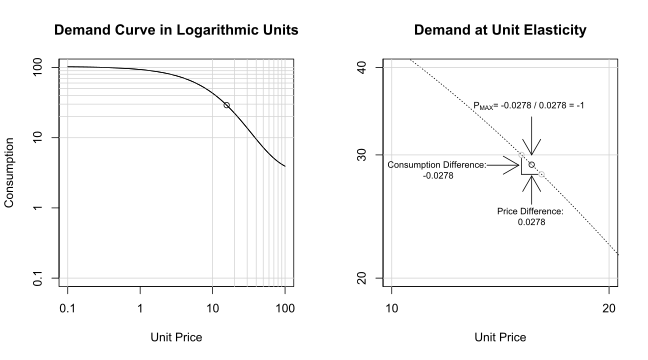
\includegraphics{plots/Figure_1-1} \end{center}

\subsubsection{Figure 2. Model Slope and Modified Loss
Function}\label{figure-2.-model-slope-and-modified-loss-function}

\begin{center}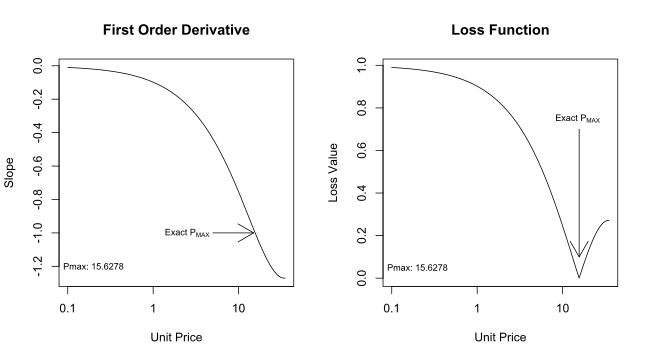
\includegraphics{plots/Figure_2-1} \end{center}

\subsubsection{Figure 3. Box Plot and Unit Elasticity
Distribution}\label{figure-3.-box-plot-and-unit-elasticity-distribution}

\begin{center}\includegraphics{plots/Figure_3-1} \end{center}

\subsubsection{Figure 4. Comparison of Exact and Approximated PMAX
Methods}\label{figure-4.-comparison-of-exact-and-approximated-pmax-methods}

\begin{center}\includegraphics{plots/Figure_4-1} \end{center}


\end{document}
